\chapter{Nombres complexes}
\label{chap:complexes}
\minitoc
\minilof
\minilot

Les nombres complexes sont présentés dans ce chapitre. L'ensemble des nombres complexes forme une extension de l'ensemble des nombres réels. Les complexes permettent notamment de définir des solutions à toutes les équations polynomiales à coefficients réels.

La première section se focalise sur leur définition et leurs propriétés. On s'intéresse ensuite à la trigonométrie en utilisant les complexes. Les équations du second degré sont ensuite résolues grâce aux complexes. L'exponentielle complexe est ensuite présentée puis l'application des complexes en géométrie plane est exposée.

\section{Corps des nombres complexes}
\label{sec:corpsdescomplexes}
La construction de ce corps est hors programme. On le définit tel quel.
\begin{defdef}
  L'ensemble des complexes est défini par
  \begin{equation}
    \C = \enstq{x+ \ii y}{(x,y)\in \R},
  \end{equation}
  tel que \(\ii^2=-1\).
\end{defdef}
\emph{Remarque} L'unité imaginaire \(\ii\) est souvent notée \(j\) en physique (pour ne pas confondre avec l'intensité). L'ensemble des complexes est muni de deux lois :
\begin{itemize}
\item l'addition, notée \(+\);
\item la multiplication, notée \(\times\) ou \(\cdot\).
\end{itemize}
%
\begin{prop} Tous les réels sont complexes, c'est-à-dire~:
  \begin{equation}
    \R \subset \C.
  \end{equation}
  Les lois de \(\R\) coïncident avec les lois sur \(\C\).
\end{prop}
%
\begin{prop}
  \((\C,+)\) est un groupe commutatif. C'est-à-dire que~:
  \begin{itemize}
  \item la loi \(+\) est associative,
    \begin{equation}
      \forall (x,y,z) \in \C^3 \quad x+(y+z)=(x+y)+z;
    \end{equation}
  \item la loi \(+\) est commutative,
    \begin{equation}
      \forall (x,y) \in \C^2 \quad x+y=y+x;
    \end{equation}
  \item \(\C\) admet un neutre pour \(+\)~: c'est \(0\);
  \item tout élément de \(\C\) est inversible par \(+\) et l'opposé de tout complexe \(x\) et \(-x\).
  \end{itemize}
\end{prop}
%
\begin{prop}
  \((\C,+,\times)\) est un anneau commutatif. C'est-à-dire que \((\C,+)\) est un groupe commutatif et que
  \begin{itemize}
  \item \(\times\) est associative;
  \item \(\times\) admet un élément neutre noté \(1\);
  \item \(\times\) est distributive sur \(+\)~:
    \begin{equation}
      \forall (a,b,c) \in \C^3 \quad a \times (b+c)=a \times b+ a \times c.
    \end{equation}
\end{itemize}
\end{prop}
%
\begin{prop}
  Pour tout complexe \(z \in \C\), il existe un unique couple de réels \((x,y) \in \R^2\) tel que \(z=x+\ii y\). C'est-à-dire que l'application
  \begin{equation}
    \fonction{\varphi}{\R^2}{\C}{(x,y)}{x+\ii y}
  \end{equation}
  est bijective.
\end{prop}
\emph{Interprétation géométrique~:} L'application $\varphi$ peut être vue comme une ``correspondance'' entre $\C$ et le plan $\R^2$, voir la figure~\ref{fig:complexe}.
\begin{figure}
    \centering
    \includegraphics[scale=0.7]{./Complexes.png}
    \label{fig:complexe}
    \caption{Représentation géométrique des complexes}
\end{figure}
\begin{proof}[Unicité]
  S'il existe deux couples de réels \((x,y),(x',y')\) tels que
  \begin{equation}
    x'+\ii y'=x +\ii y,
  \end{equation}
  alors
  \begin{equation}
    \underbrace{(x-x')^2}_{\geqslant 0}=\underbrace{-(y'-y)^2}_{\leqslant 0}.
  \end{equation}
  Finalement
  \begin{equation}
    (x-x')^2=(y'-y)^2=0.
  \end{equation}
\end{proof}
\begin{proof}[Existence]
  Par définition de l'ensemble des complexes, pour un complexe \(z\) donné, il existe toujours un couple de réels qui lui est associé.
\end{proof}
%
On appelle le réel \(x\) la partie réelle du complexe \(z\), \(x=\Re(z)\) et on appelle le réel \(y\) la partie imaginaire du complexe \(z\), \(y=\Im(z)\).
%
\begin{prop}
  Soient des complexes \(z\) et \(z'\) puis un réel \(\lambda\), alors
  \begin{gather}
    \Re(z+z')=\Re(z)+\Re(z'), \\
    \Im(z+z')=\Im(z)+\Im(z'),\\
    \Re(\lambda z)=\lambda \Re(z),\\
    \Im(\lambda z)=\lambda \Im(z).
  \end{gather}
\end{prop}
%
\emph{Un complexe n'a pas de signe}. On note \(\C^*=\C \setminus \{0\}\)
%
\subsection{Conjugaison de complexe}
\label{subsec:conjugaisoncomplexe}
\begin{defdef}
  Soit \(z=x+\ii y \in \C\) avec \((x,y)\in \R\), on définit son conjugué de \(z\) noté \(\bar{z}\) par \(\bar{z}=x- \ii y\).
\end{defdef}
Les conjugués de deux complexes sont représentés dans le plan complexe sur la figure \ref{fig:conjugueComplexe}.
\begin{figure}
    \centering
    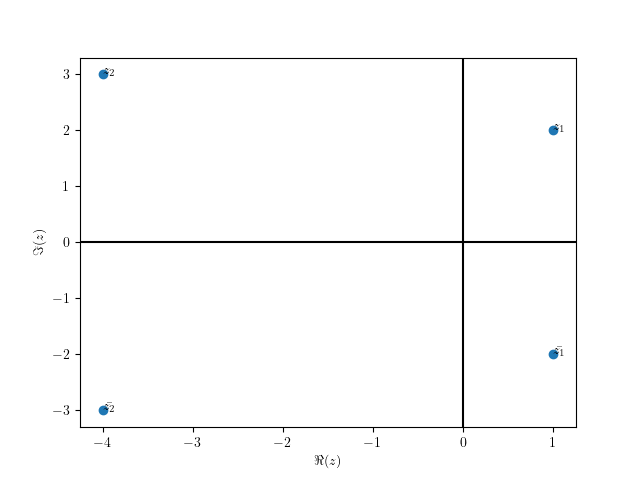
\includegraphics[scale=0.7]{conjugue.png}
    \caption{Représentation dans le plan complexe du conjugué de deux complexes $z_1$ et $z_2$}
    \label{fig:conjugueComplexe}
\end{figure}
%
\begin{prop}
  Soient des complexes \(z\) et \(z'\), alors
  \begin{gather}
    \bar{z+z'}=\bar{z} + \bar{z'}; \\
    \bar{z \cdot z'}=\bar{z} \cdot \bar{z'}; \\
    \bar{\bar{z}}=z.
  \end{gather}
\end{prop}
\begin{prop}
  pour tout complexe \(z\) on a
  \begin{gather}
    \Re(z)=\frac{z+\bar{z}}{2};\\
    \Im(z)=\frac{z-\bar{z}}{2 \ii};\\
    z \in \R \iff z=\bar{z};\\
    z \in \ii\R \iff z=-\bar{z}.
  \end{gather}
\end{prop}
%
\subsection{Module d'un complexe}
\label{subsec:modulecomplexe}
\begin{prop}
  Soit un complexe \(z\), alors \(z \bar{z} \in \R\) et \(z \bar{z}=0 \iff z = 0\).
\end{prop}
\begin{proof}
  Soit un complexe \(z\), notons \(x\) sa partie réelle et \(y\) sa partie imaginaire, alors
  \begin{equation}
    z \bar{z}=x^2+y^2 \geqslant 0,
  \end{equation}
  et
  \begin{equation}
    z \bar{z}=0 \iff x^2+y^2=0 \iff x=y=0 \iff z=0.
  \end{equation}
\end{proof}
%
\begin{defdef}
  Pour tout complexe \(z\), on définit le module de \(z\) par \(\abs{z}=\sqrt{z \bar{z}}\).
\end{defdef}
%
On peut représenter le module dans le plan complexe par la figure \ref{fig:moduleComplexe}
\begin{figure}
    \centering
    \includegraphics[scale=0.7]{module_complexe.png}
    \caption{Représentation dans le plan complexe du module}
    \label{fig:moduleComplexe}
\end{figure}
%
\begin{prop}
  Soient \(z\) et \(z'\) deux complexes, alors
  \begin{gather}
    \abs{z}=\abs{\bar{z}}; \\
    \abs{z \cdot z'}=\abs{z} \cdot \abs{z'}; \\
    \abs{z+z'}\leqslant\abs{z}+\abs{z'}.
  \end{gather}
  Avec égalité s'il existe un réel \(\lambda\) tel que \(z'=\lambda z\).
\end{prop}
\begin{proof}
  \begin{equation}
    (\abs{z}+\abs{z'})^2-\abs{z+z'}^2
    =(\sqrt{z \bar{z}} +\sqrt{z' \bar{z'}})^2 - (z+z')(\bar{z+z'})
    =2 \sqrt{z \bar{z} z' \bar{z'}} - z \bar{z'} - z'\bar{z}
  \end{equation}
  On pose \(u=z \bar{z'}\) et on a
  \begin{equation}
    (\abs{z}+\abs{z'})^2-\abs{z+z'}^2=2 \abs{u}-2 \Re(u) \geqslant 0.
  \end{equation}
  On a montré que \((\abs{z}+\abs{z'})^2 \geqslant \abs{z+z'}^2\) et comme ce sont des nombres positifs, en appliquant la racine carré~\footnote{qui est une fonction croissante}, on obtient l'inégalité triangulaire.

  \emph{Cas d'égalité}~: Notons ici que \(\frac{z'}{z}=x + \ii y\) avec \(x\) et \(y\) deux réels. On va montrer que l'égalité est vraie si et seulement si \(y=0\) et \(x \geqslant 0\).
  \begin{align}
    \abs{z+z'}=\abs{z}+\abs{z'} &\iff \abs{1+\frac{z'}{z}}^2=\left(1+\abs{\frac{z'}{z}}\right)^2 \\
    &\iff \abs{1+x+\ii y}^2 = (1+ \abs{x+ \ii y})^2 \\
    &\iff (1+x)^2+y^2 = (1+\sqrt{x^2+y^2})^2 \\
    &\iff 1+2x+x^2+y^2 = 1 + 2\sqrt{x^2+y^2} + x^2+y^2 \\
    &\iff x = \sqrt{x^2+y^2}\\
    &\iff y=0 \text{~et~} x \geqslant 0.
  \end{align}
\end{proof}
%
\begin{prop}
  Tout complexe \(z\) non nul admet un unique inverse, c'est \(\frac{\bar{z}}{\abs{z}^2}\).
\end{prop}
\begin{proof}
  D'une part
  \begin{equation}
    z \cdot \frac{\bar{z}}{\abs{z}^2}=\frac{z \bar{z}}{\abs{z}^2}=1,
  \end{equation}
  et d'autre part si \(z\cdot z'=z'\cdot z=1\) alors \(z'\cdot z\cdot \frac{\bar{z}}{\abs{z}^2}=z'\). Comme \(z\cdot z'=1\), on a \( \frac{\bar{z}}{\abs{z}^2}\cdot z\cdot z'=\frac{\bar{z}}{\abs{z}^2}\) donc \(z'=\frac{\bar{z}}{\abs{z}^2}\).
\end{proof}
En pratique, on multiplie par le complexe conjugué : \(\frac{1}{x+\ii y}=\frac{x -\ii y}{x^2+y^2}\).
%
\begin{prop}
  \((\C,+,\times)\) est un anneau commutatif intègre. \((\C^*,+,\times)\) est aussi un corps commutatif.
\end{prop}
%
\begin{prop}
  Soient un complexe \(z\) non nul et un complexe \(z'\) quelconque, alors on a
  \begin{gather}
    \bar{\frac{1}{z}}=\frac{1}{\bar{z}}; \\
    \abs{\frac{1}{z}}=\frac{1}{\abs{z}}; \\
    \bar{\frac{z'}{z}} = \frac{\bar{z'}}{\bar{z}};\\
    \abs{\frac{z'}{z}}=\frac{\abs{z'}}{\abs{z}}.
  \end{gather}
\end{prop}
%
\begin{defdef}
  Soient un complexe \(a\) et un réel positif \(r\), on définit le disque ouvert de centre \(a\) et de rayon \(r\), noté \(D_o(a,r)\), par~:
  \begin{equation}
    D_o(a,r)=\enstq{z\in\C}{\abs{z-a}<r},
  \end{equation}
  et on définit le disque fermé, noté \(D_f(a,r)\), par~:
  \begin{equation}
    D_f(a,r)=\enstq{z\in\C}{\abs{z-a}\leqslant r}.
  \end{equation}
\end{defdef}
%
\subsection{Plan complexe}
\label{subsec:plancomplexe}
%
Soit \(\P\) le plan euclidien muni d'un repère orthonormé \((O,\vect{u}, \vect{v})\). Si \(M\) est un point du plan \(\mathcal{P}\) de coordonnées \((x,y)\) dans le repère \((O,\vect{u}, \vect{v})\), on appelle l'affixe de \(M\), le complexe \(z=x + \ii y\). Pour tous complexe \(z\), il existe un point du plan \(\mathcal{P}\) d'affixe \(z\), c'est \(M(z)\). L'application \(\fonction{\varphi}{\C}{\P}{z}{M(z)}\) est une bijection. Cette bijection permet ``d'identifier'' \(\C\) et le plan \(\P\). Dans ce cadre~:
\begin{itemize}
\item \(M(\bar{z})\) est le symétrique de \(M(z)\) par rapport à l'axe \((O,\vect{u})\);
\item \(M(-z)\) est le symétrique de \(M(z)\) par rapport au point O;
\item le module de \(z\), \(\abs{z}\) est la distance de O à \(M(z)\);
\item \(\abs{z-z'}\) est la distance entre \(M(z)\) et \(M(z')\);
\item l'inégalité triangulaire dit que la distance de \(M(z)\) à \(M(z')\) est inférieure ou égale à la somme de la distance entre O et \(M(z)\) et de la distance entre O et \(M(z')\);
\item \(D_o(a,r)\) est l'ensemble des points \(M(z)\) dont la distance au point \(A(a)\) est strictement inférieure à \(r\).
\end{itemize}
Si \(\vect{a}\) est un vecteur on définit son affixe comme l'affixe du point \(M\) tel que \(\vect{a}=\vect{OM}\).
% La figure~\ref{planP} représente ces points.
% \begin{figure}
%   \centering
%   \begin{tikzpicture}
%     \draw [thin, gray] (-4,-4) grid[step=0.5] (4,4);

%     \draw[->] (-4,0) -- (4,0);
%     \draw[->] (0,-4) -- (0,4);

%     \coordinate (O) at (0,0);
%     \coordinate (M) at (2,2);
%     \coordinate (moinsM) at (-2,-2);
%     \coordinate (Mbar) at (2,-2);
%     \coordinate (Mprime) at (-1,3);

%     \draw (O) node[below left]{\(O\)};
%     \draw (M) node {\(\bullet\)}; \draw (M) node[below] {\(M(z)\)};
%     \draw (moinsM) node {\(\bullet\)}; \draw (moinsM) node[below] {\(M'(-z)\)};
%     \draw (Mbar) node {\(\bullet\)}; \draw (Mbar) node[below] {\(\bar{M}(\bar{z})\)};
%     \draw (Mprime) node {\(\bullet\)}; \draw (Mprime) node[below] {\(M'(z')\)};
%     \draw (3,0) node[below] {\(\vect{u}\)};
%     \draw (0,3) node[right] {\(\vect{v}\)};
%     \draw[>=latex,->] (M) -- (Mprime);

%   \end{tikzpicture}
%   \label{planP}
%   \caption{Représentation du plan complexe}
% \end{figure}
%
\section{Groupe des complexes de module 1}
\label{sec:groupeU}
\subsection{Définitions et premières propriétés}
\label{subsec:groupeU-defetprop}
\begin{defdef}
  Le groupe des complexes de module 1, noté \(\U\), est~:
  \begin{equation}
    \U=\enstq{z \in \C}{\abs{z}=1}.
  \end{equation}
  Géométriquement parlant, \(\U\) est le cercle de centre \(O\) et de rayon \(1\).
\end{defdef}
%
\begin{prop}
  Soit un complexe \(z\), alors
  \begin{equation}
    z \in \U \iff z \cdot \bar{z}=1 \iff \bar{z}=\frac{1}{z}.
  \end{equation}
\end{prop}
%
\begin{prop}
  \((\U, \times)\) est un groupe commutatif (ou abélien), c'est-à-dire que~:
  \begin{enumerate}
  \item \(\forall (z,z') \in \U^2 \quad zz' \in \U\);
  \item la loi \(\times\) est associative et commutative;
  \item \(\U\) admet \(1\) comme élément neutre pour \(\times\);
  \item tout élément de \(\U\) admet un inverse dans \(\U\).
  \end{enumerate}
\end{prop}
\begin{proof}
  \begin{enumerate}
  \item Soit deux complexes \(z\) et \(z'\) de \(\U\), alors \(\abs{zz'}=\abs{z}\abs{z'}=1\) donc \(zz' \in \U\);
  \item puisque la loi \(\times\) est associative et commutative dans \(\C\), elle l'est dans \(\U\);
  \item le module de 1 est égal à 1 donc \(1 \in \U\);
  \item soit un complexe \(z\) de \(\U\), comme son module vaut 1, il est non nul et il admet un inverse et \(\abs{\frac{1}{z}}=\frac{1}{\abs{z}}=1\) donc l'inverse est dans \(\U\).
  \end{enumerate}
\end{proof}
%
\begin{prop}\label{prop:expsurj}
  Soit un complexe \(z\) de \(\U\), alors il existe un réel \(\theta\) ---~unique modulo \(2\pi\)~--- tel que \(z=\cos\theta +\ii\sin\theta\).
\end{prop}
\begin{proof}[Existence]
  Soit un complexe \(z\) de \(\U\), notons \(x\) et \(y\) respectivement sa partie réelle et sa partie imaginaire. Alors \(x^2+y^2=\abs{z}^2=1\), donc d'après le théorème~\ref{chap1-theo:thetasin} il existe un unique \(\theta_0 \in \intervalleof{-\pi}{\pi}\) tel que \(x=\cos\theta_0\) et \(y=\sin\theta_0\).
\end{proof}
\begin{proof}[Unicité]
  Montrons l'unicité modulo \(2\pi\) : Soit deux réels \(\theta\) et \(\theta'\) vérifiant  \(x=\cos \theta=\cos \theta'\) et \(y=\sin \theta = \sin \theta'\). Il existe deux entiers relatifs \(k\) et \(l\) tels que \(\theta +2k \pi \in \intervalleof{-\pi}{\pi}\) et \(\theta' +2kl \pi \in \intervalleof{-\pi}{\pi}\). Donc on a \(\theta_0=\theta + 2k \pi=\theta'+2l \pi\), soit encore \(\theta-\theta'=(l-k) 2\pi\), c'est à dire \(\theta \equiv \theta' [2\pi]\).
\end{proof}
%
\begin{defdef}[Exponentielle complexe]
  Pour tout réel \(\theta\), on note
  \begin{equation}\
    \expc{}{\theta}=\cos\theta +\ii\sin\theta.
  \end{equation}
\end{defdef}
%
\begin{prop}
  L'application \(\fonction{\psi}{\R}{\U}{\theta}{\expc{}{\theta}}\) est un morphisme du groupe \((\R,+)\) sur le groupe \((\U,\times)\).
\end{prop}
\begin{proof}
  pour tout réel \(\theta\), on a bien
  \begin{equation}
    \abs{\expc{}{\theta}}=\sqrt{\cos^2 \theta + \sin^2 \theta}=1,
  \end{equation}
  donc \(\psi(\theta) \in \U\). Ensuite,
  \begin{align}
    \psi(\theta +\theta') = &\cos(\theta +\theta') + \ii \sin(\theta + \theta')\\
    =&\cos \theta \cos \theta' - \sin \theta \sin \theta' +\ii(\cos \theta \sin \theta' + \sin \theta \cos \theta')\\
    =&(\cos \theta + \ii \sin \theta)(\cos \theta' + \ii \sin \theta')\\
    =&\psi(\theta) \psi(\theta')
  \end{align}
\end{proof}
%
\begin{prop} Soient deux réels \(\theta\) et \(\theta'\) et un entier relatif \(n\), alors~:
  \begin{gather}
    \expc{}{(\theta-\theta')}=\frac{\expc{}{\theta}}{\expc{}{\theta'}};\\
    \expc{}{n \theta}=(\expc{}{\theta})^n;\\
    \cos \theta = \frac{\e^{\ii \theta}+\e^{-\ii\theta}}{2} \quad \sin \theta = \frac{\e^{\ii \theta}-\e^{-\ii\theta}}{2\ii}.
  \end{gather}
\end{prop}
\begin{proof}
	La première égalité découle directement de la proposition précédente, \(\psi\) est un morphisme de \((\R,+)\) sur \((\U,\times)\). Ensuite, la deuxième égalité se démontre par récurrence et la dernière découle directement de la définition de l'exponentielle complexe.
\end{proof}

Soient un entier naturel \(n\) non nul et \(\theta \in \R \setminus 2\pi\Z\). La somme vaut~:
\begin{align}
  \sum_{k=0}^n \cos(k\theta) =& \frac{1}{2} \sum_{k=0}^n (\expc{}{k \theta} + \expc{}{-k \theta})\\
  =&\frac{1}{2} \left[\frac{1-\expc{}{(n+1)\theta}}{1-\expc{}{\theta}}\right] + \frac{1}{2} \left[\frac{1-\expc{}{(-(n+1) \theta)}}{1-\expc{}{-\theta}}\right]\\
  =&\frac{1}{2} \left[\frac{\expc{}{(n+1) \frac{\theta}{2}}}{\expc{}{\frac{\theta}{2}}} \left(\frac{\expc{}{\left(-(n+1) \frac{\theta}{2}\right)}-\expc{}{(n+1) \frac{\theta}{2}}}{\expc{}{\left(-\frac{\theta}{2}\right)} - \expc{}{\frac{\theta}{2}}} \right)\right] \notag + \frac{1}{2} \left[\frac{\expc{}{\left(-(n+1) \frac{\theta}{2}\right)}}{\expc{}{\left(-\frac{\theta}{2}\right)}} \left(\frac{\expc{}{(n+1) \frac{\theta}{2}}-\expc{}{\left(-(n+1) \frac{\theta}{2}\right)}}{\expc{}{\frac{\theta}{2}} - \expc{}{\left(-\frac{\theta}{2}\right)}} \right)\right] \\
  =& \frac{1}{2} \frac{\sin \left(\frac{(n+1)\theta}{2} \right)}{\sin \left( \frac{\theta}{2} \right)} \left[\expc{}{n \frac{\theta}{2}} +\expc{}{\left(-n \frac{\theta}{2}\right)} \right] \\
  =& \frac{\sin \left(\frac{(n+1)\theta}{2} \right)}{\sin \left( \frac{\theta}{2} \right)} \cos \left( \frac{n\theta}{2} \right).
\end{align}
%
Car
\begin{equation}
  \forall (a,b) \in \R^2 \quad \expc{}{a}-\expc{}{b}=2\ii \sin\left(\frac{a-b}{2}\right)\expc{}{\frac{(a+b)}{2}}.
\end{equation}

\begin{prop}
  L'application \(\psi\) est  \(2\pi\)-périodique et surjective. C'est-à-dire que pour tout complexe \(z\) de \(\U\), il existe un réel \(\theta\) tel que \(z=\expc{}{\theta}\). On a
  \begin{gather}
    \forall \theta \in \R \quad \psi(-\theta)=\bar{\psi(\theta)};\\
    \forall (\theta, \theta') \in \R^2 \quad \expc{}{\theta}=\expc{}{\theta'} \iff \congru{\theta}{\theta'}{2\pi}.
  \end{gather}
\end{prop}
\begin{proof}
  \begin{itemize}
  \item \(\psi\) est \(2\pi\)-périodique car \(\cos\) et \(\sin\) le sont;
  \item \(\psi\) est surjective d'après la proposition~\ref{prop:expsurj}.
  \end{itemize}
\end{proof}
%
\begin{prop}
  L'application \(\psi\) est dérivable sur \(\R\) et
  \begin{equation}
    \forall \theta \in \R \quad \psi'(\theta)=\ii \expc{}{\theta}.
  \end{equation}
\end{prop}
\begin{proof}
  Admettons qu'une fonction \(f \in \C^{\R}\) telle que \(f=x+\ii y\) avec \((x,y) \in \R^{\R} \times \R^{\R}\) est dérivable si et seulement si \(x\) et \(y\) sont dérivables sur \(\R\) et auquel cas \(f'=x' +\ii y'\). Ici, \(\psi=\cos +\ii \sin\), \(\sin\) et \(\cos\) sont dérivables alors \(\psi'=-\sin + \ii \cos=\ii (\cos +\ii \sin)=\ii \psi\).
\end{proof}
%
\subsection{Trigonométrie}
\label{subsec:complexestrigo}
\subsubsection{Polynômes de Chebychev}
\label{subsubsec:Chebychev}
\begin{defdef}
  On définit les polynômes de Chebychev en suivant ce raisonnement~:
  \begin{align}
    \cos n \theta + \ii \sin n \theta =& (\cos \theta + \ii \sin \theta)^n\\
    =& \sum_{k=0}^n \binom{n}{k} \ii^k \sin^k \theta \cos^{n-k} \theta\\
    =& \sum_{2p \leqslant n} \binom{n}{2p} (-1)^p \sin^{2p} \theta \cos^{n-2p} \theta \\ &+ \ii \sin \theta \sum_{2p +1\leqslant n} \binom{n}{2p+1} (-1)^p \sin^{2p} \theta \cos^{n-2p-1} \theta.
  \end{align}
  En remplaçant par \(\sin^2 \theta\) par \(1-\cos^2 \theta\), on obtient
  \begin{equation}
    \cos n \theta = P_n(\cos \theta) \quad \sin n \theta = \sin \theta \cdot Q_n(\cos \theta).
  \end{equation}
  \(P_n\) et \(Q_n\) sont respectivement les polynômes de Chebychev de 1\iere{} et de 2\ieme{} espèce.
\end{defdef}
%
\subsubsection{Arc moitié}
\label{subsubsec:arcmoitie}
Pour tout réel \(\theta\) non congru à \(\pi\) modulo--\(2\pi\) on pose \(t=\tan \left( \frac{\theta}{2} \right)\) alors
\begin{gather}
  \cos \theta = \dfrac{1-t^2}{1+t^2};\\
  \sin \theta = \dfrac{2t}{1+t^2}; \\
  \tan \theta = \frac{2t}{1-t^2};\\
  \e^{\ii \theta}=\frac{(1+\ii \theta)^2}{1+t^2}.
\end{gather}
La bijection \(\fonction{\varphi}{\R}{\U\setminus \{-1\}}{t}{\frac{(1+\ii \theta)^2}{1+t^2}}\) fournit un paramétrage du cercle trigonométrique privé du point \((-1,0)\).
%
\subsubsection{Linéarisation}
\label{subsubsec:linearisation}
Pour tout réel \(\theta\) on a~:
\begin{gather}
  \cos^2 \theta = \frac{1+\cos 2\theta}{2}; \\
  \sin^2 \theta = \frac{1-\cos 2\theta}{2}.
\end{gather}
Si l'exposant \(p \geqslant 3\), on utilise les formules d'Euler
\begin{gather}
  \cos^p \theta = \left(\frac{\expc{}{\theta}+\expc{}{\theta}}{2} \right)^p, \\
  \sin^p \theta = \left(\frac{\expc{}{\theta}-\expc{}{\theta}}{2 \ii} \right)^p,
\end{gather}
puis on développe avec la formule du binôme de Newton et on regroupe judicieusement les termes obtenus.
%
\subsubsection{Transformations de sommes en produits}
\label{subsubsec:sommeprod}
La transformation de produit en somme s'effectue en suivant le raisonnement suivant~:
\begin{align}
  \expc{}{a}+\expc{}{b} &= \expc{}{\frac{a+b}{2}} \left(\expc{}{\frac{a-b}{2}} + \expc{}{\frac{b-a}{2}}\right) \\
  & =  \expc{}{\frac{a+b}{2}} 2\cos \left(\frac{a-b}{2} \right).\\
  \expc{}{a}-\expc{}{b} &= \expc{}{\frac{a+b}{2}} \left( \expc{}{\frac{a-b}{2}} - \expc{}{\frac{b-a}{2}} \right) \\
  & =  \expc{}{\frac{a+b}{2}} 2 \ii \sin \left( \frac{a-b}{2} \right).
\end{align}
On identifie la partie réelle et la partie imaginaire pour écrire que
\begin{align}
  & \cos a + \cos b = 2 \cos \left( \frac{a+b}{2} \right) \cos \left(\frac{a-b}{2} \right);\\
  & \sin a + \sin b = 2 \sin \left( \frac{a+b}{2} \right) \cos \left(\frac{a-b}{2} \right);\\
  & \cos a - \cos b = -2 \sin \left( \frac{a+b}{2} \right) \sin \left(\frac{a-b}{2} \right);\\
  & \sin a - \sin b = 2 \cos \left( \frac{a+b}{2} \right) \sin \left(\frac{a-b}{2} \right).
\end{align}
On peut retrouver les formules de transformation de sommes en produits, puis de produits en sommes.
%
\subsection{Argument d'un complexe}
\label{subsec:argumentcomplexe}
Soit \(z\) un complexe non nul. Le complexe \(\frac{z}{\abs{z}}\) est de module 1, donc il existe un réel \(\theta\) tel que \(\frac{z}{\abs{z}}=\expc{}{\theta}\)
\begin{defdef}
  Si \(z\) est un complexe non nul, on appelle argument de \(z\) tout réel \(\theta\) tel que \(z=\expc{\abs{z}}{\theta}\).  Le réel \(\theta\) est défini modulo-\(2\pi\), on note \(\congru{\arg(z)}{\theta}{2\pi}\). L'unique réel \(\theta \in \intervalleof{-\pi}{\pi}\), qui est un argument de \(z\), est l'argument principal de \(z\), noté \(\Arg(z)\).
\end{defdef}
L'écriture \(z=\expc{\abs{z}}{\theta}\) avec \(\theta \in \R\) est appelée forme trigonométrique du complexe non nul \(z\).

\emph{Remarque}~: Si on ne sait pas que le complexe est non nul, on ne parle ni d'argument ni de forme trigonométrique.
\begin{prop}
  Soit un complexe \(z\) non nul, alors
  \begin{equation}
    \forall (\theta, \theta') \in \R^2 \ \forall (\rho, \rho') \in \Rpluss \times \Rpluss \quad z=\expc{\rho}{\theta}=\expc{\rho'}{\theta'} \iff
    \begin{cases}
      \rho = \rho' = \abs{z} \\
      \congru{\theta}{\theta'}{2\pi}
    \end{cases}.
  \end{equation}
\end{prop}
\begin{proof}
  La preuve de cette proposition découle directement de la définition.
\end{proof}
%
\begin{prop}
  Soient deux complexes non nuls \(z\) et \(z'\) et un entier relatif \(n\), alors
  \begin{gather}
    \congru{\arg(z)}{0}{\pi} \iff z \in \R^*;\\
    \congru{\arg(z)}{\frac{\pi}{2}}{\pi} \iff z \in \ii\R^{*};\\
    \congru{\arg(\bar{z})}{-\arg(z)}{2\pi};\\
    \congru{\arg(z z')}{\arg(z) + \arg(z')}{2\pi};\\
    \congru{\arg(z^n)}{n \arg(z)}{2\pi};\\
    \congru{\arg \left(\frac{z}{z'} \right)}{\arg(z) - \arg(z') }{2\pi};\\
    \congru{\arg(-z)}{\pi + \arg(z)}{2\pi}.
  \end{gather}
\end{prop}
\begin{proof}
  La preuve s'articule en cinq parties~:
  \begin{enumerate}
  \item \(\congru{\arg(z)}{0}{\pi} \iff z = \pm \abs{z}\);
  \item \(\congru{\arg(z)}{\frac{\pi}{2}}{\pi} \iff z = \pm \ii \abs{z}\);
  \item si \(z=\expc{\abs{z}}{\theta}\), alors \(\bar{z}=\bar{\expc{|z|}{\theta}}=\expc{|z|}{(-\theta)}\) donc \(\congru{\arg(\bar{z})}{-\arg(z)}{2\pi}\);
  \item si on met \(z\) et \(z'\) sous forme trigonométrique, on retrouve les formules 4, 5 et 6 par le calcul;
  \item puisque \(-1=\expc{}{\pi}\), on a bien la dernière formule.
  \end{enumerate}
\end{proof}

\emph{Interprétation géométrique}~: Dans le plan complexe muni d'un repère \((O,\vect{u}, \vect{v})\), \(\arg(z)\) représente une mesure de l'angle \(\widehat{\vect{u}, \vect{OM}(z)}\). Plus généralement, si \(a\), \(b\) et \(c\) sont trois complexes distincts affixes respectives des points \(A\), \(B\) et \(C\) alors \(\arg\left(\frac{b-a}{c-a}\right)\) représente une mesure de l'angle \((\widehat{\vect{BA},\vect{BC}})\). Donc \(A\), \(B\) et \(C\) sont alignés si et seulement si le complexe \(\frac{b-a}{c-a}\) est un réel non nul.
%
\subsection{Racines \(n\)\iemes{} de l'unité}
\label{subsec:racineunite}
\begin{defdef}
  Soit un entier naturel non nul \(n\), on appelle racine \(n\)\iemes{} de l'unité tout complexe \(z\) tel que \(z^n=1\). L'ensemble de ces complexes est noté \(\U_n\)
\end{defdef}
\begin{prop}
  Soit un entier naturel \(n\) non nul, alors
  \begin{equation}
    \U_n=\enstq{\expc{}{\frac{2 \pi k}{n}}}{k\in\intervalleentier{0}{n-1}}.
  \end{equation}
  Cet ensemble est de cardinal \(n\).
\end{prop}
\begin{proof}
  Soit un complexe \(z\) de \(\U_n\) noté \(\expc{\rho}{\theta}\), alors comme \(z^n=1\) on a \(\rho=1\) et \(\congru{n\theta}{0}{2\pi}\) c'est à dire que \(z \in \enstq{\expc{}{\frac{2k\pi}{n}}}{k \in \Z}\).
  \begin{itemize}
  \item Soient deux entiers relatifs \(k\) et \(l\) de \(\intervalleentier{0}{n-1}\) alors \(\abs{\frac{2\pi}{n}k - \frac{2\pi}{n}l} \leqslant 2\pi\) donc \(\expc{}{\frac{2\pi k}{n}} \neq \expc{}{\frac{2\pi l}{n}}\). Il y a donc \(n\) racines distinctes.
  \item Soit un entier relatif \(k\), il existe un entier \(l \in \intervalleentier{0}{n-1}\) tel que \(\congru{k}{l}{n}\)~:
      Puisque si on définit \(k\) tel que \(p=\Ent\left( \frac{k}{n} \right)\) alors
      \begin{align}
        np \leqslant & k < np +n \\
        0 \leqslant & k-np \leqslant n-1 <n.
      \end{align}
    \end{itemize}
    Alors on a démontré que \(\U_n \subset \enstq{\expc{}{\frac{2k\pi}{n}}}{k \in \Z}\), on déduit l'autre inclusion en vérifiant que tous les éléments de \(\enstq{\expc{}{\frac{2k\pi}{n}}}{k \in \Z}\) élevés à la puissance \(n\) font 1.
\end{proof}

\emph{Interprétation géométrique}~: Les points d'affixes \(z \in \U_n\) forment les sommets d'un polygone régulier à \(n\) cotés centré en O dont l'un des sommet est \(1\). Les représentations géométriques des ensembles \(\U_3\) jusqu'à \(\U_{14}\) sont données par le figure~\ref{fig:racinesnieme}.
\begin{figure}
    \begin{subfigure}{.3\textwidth}
      \centering
      % include first image
      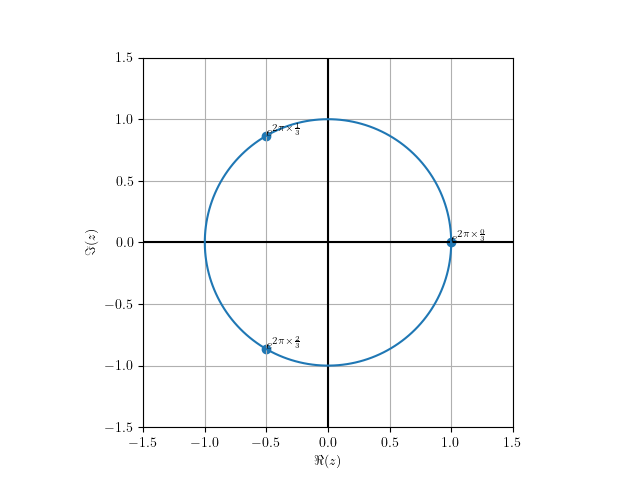
\includegraphics[scale=.33]{U_3.png}  
      \caption{$\U_3$}
      \label{fig:U3}
    \end{subfigure}
    \begin{subfigure}{.3\textwidth}
      \centering
      % include second image
      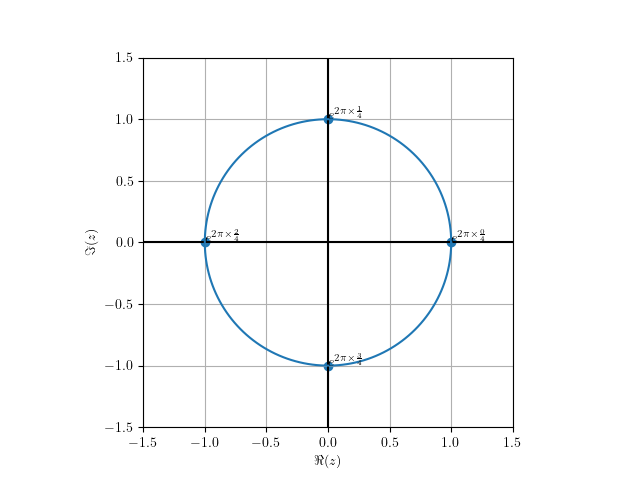
\includegraphics[scale=.33]{U_4.png}  
      \caption{$\U_4$}
      \label{fig:U4}      
    \end{subfigure}
    \begin{subfigure}{.3\textwidth}
      \centering
      % include second image
      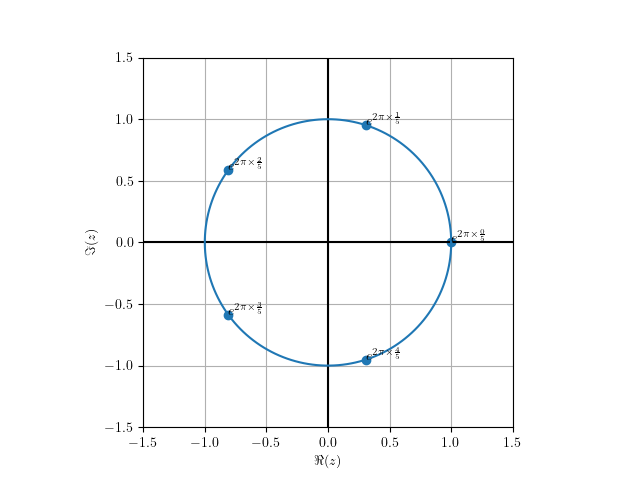
\includegraphics[scale=.33]{U_5.png}  
      \caption{$\U_5$}
      \label{fig:U5}      
    \end{subfigure}
    \newline
    \begin{subfigure}{.3\textwidth}
      \centering
      % include second image
      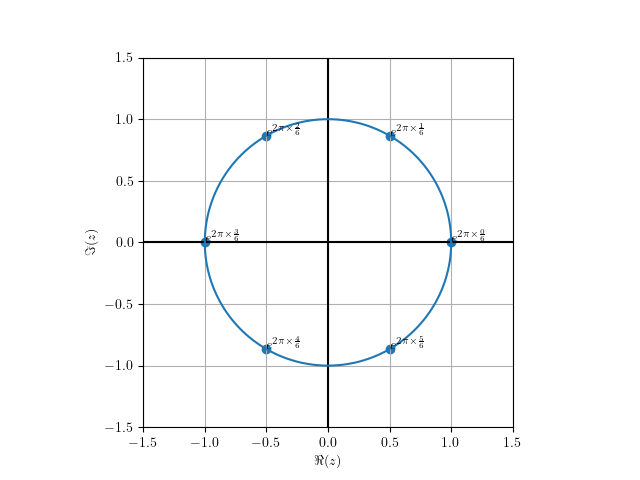
\includegraphics[scale=.33]{U_6.png}  
      \caption{$\U_6$}
      \label{fig:U6}      
    \end{subfigure}
    \begin{subfigure}{.3\textwidth}
      \centering
      % include first image
      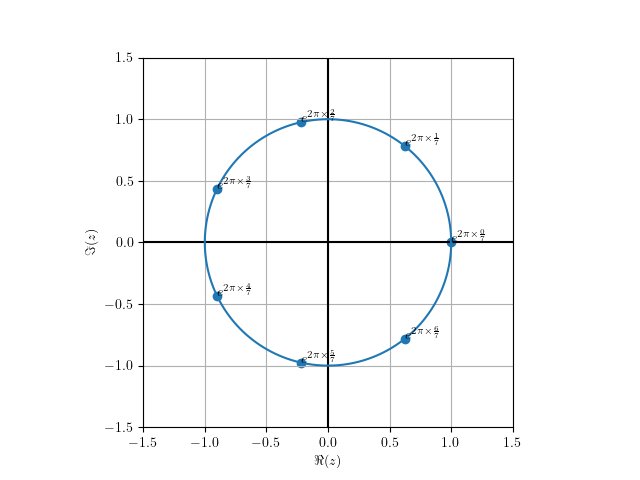
\includegraphics[scale=.33]{U_7.png}  
      \caption{$\U_7$}
      \label{fig:U7}
    \end{subfigure}
    \begin{subfigure}{.3\textwidth}
      \centering
      % include second image
      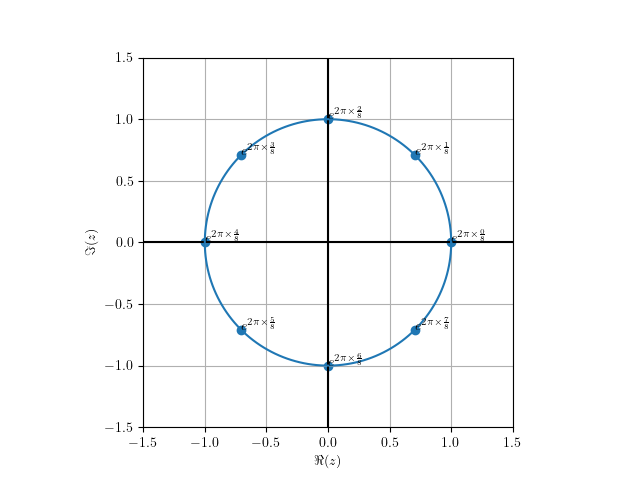
\includegraphics[scale=.33]{U_8.png}  
      \caption{$\U_8$}
      \label{fig:U8}      
    \end{subfigure}
    \newline
    \begin{subfigure}{.3\textwidth}
      \centering
      % include second image
      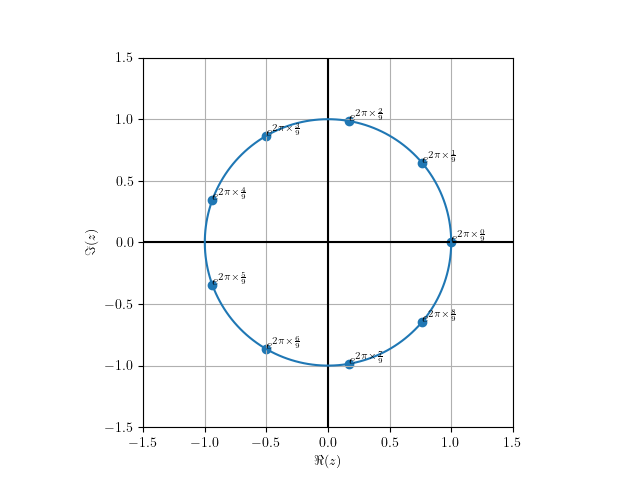
\includegraphics[scale=.33]{U_9.png}  
      \caption{$\U_9$}
      \label{fig:U9}      
    \end{subfigure}
    \begin{subfigure}{.3\textwidth}
      \centering
      % include second image
      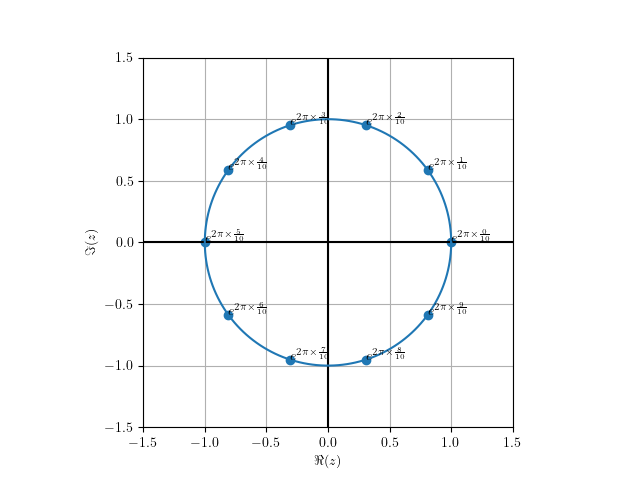
\includegraphics[scale=.33]{U_10.png}  
      \caption{$\U_{10}$}
      \label{fig:U10}
    \end{subfigure}  
    \begin{subfigure}{.3\textwidth}
      \centering
      % include first image
      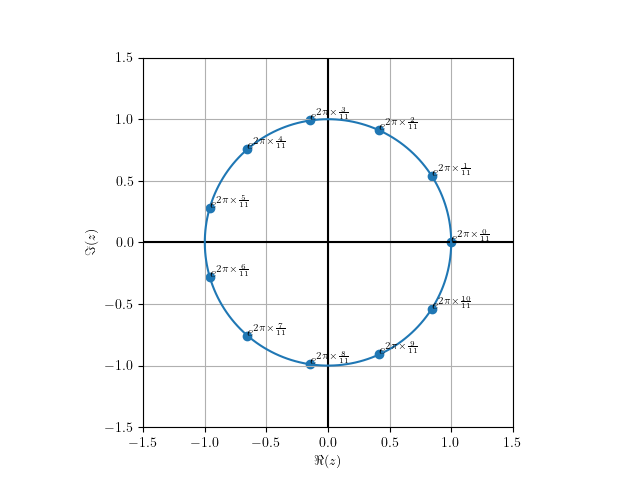
\includegraphics[scale=.33]{U_11.png}  
      \caption{$\U_{11}$}
      \label{fig:U11}
    \end{subfigure}
    \newline
    \begin{subfigure}{.3\textwidth}
      \centering
      % include second image
      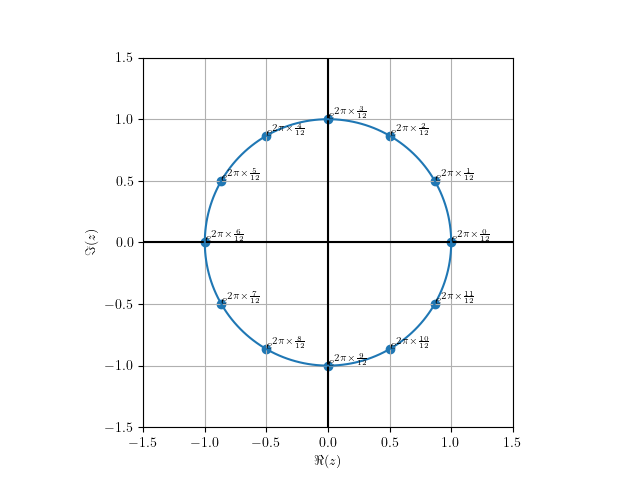
\includegraphics[scale=.33]{U_12.png}  
      \caption{$\U_{12}$}
      \label{fig:U12}      
    \end{subfigure}
    \begin{subfigure}{.3\textwidth}
      \centering
      % include second image
      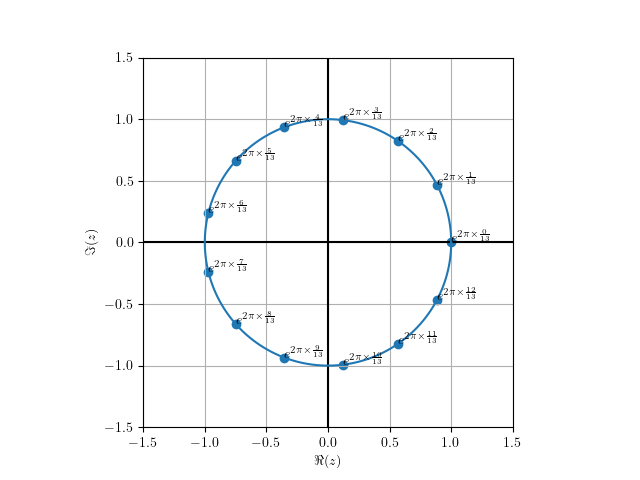
\includegraphics[scale=.33]{U_13.png}  
      \caption{$\U_{13}$}
      \label{fig:U13}      
    \end{subfigure}
    \begin{subfigure}{.3\textwidth}
      \centering
      % include second image
      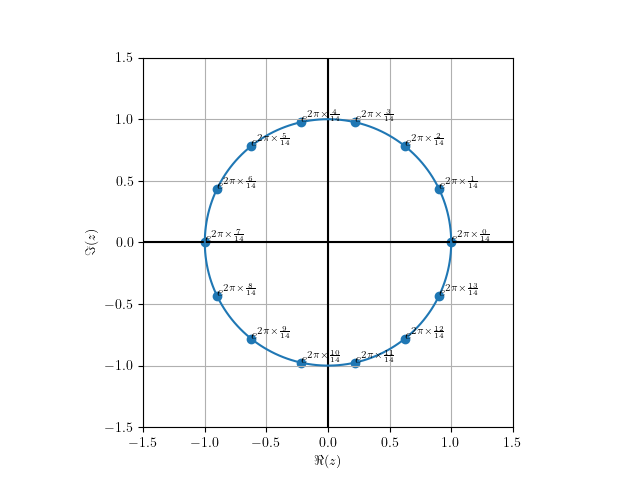
\includegraphics[scale=.33]{U_14.png}  
      \caption{$\U_{14}$}
      \label{fig:U14}
    \end{subfigure}
 \caption{Représentations graphique de $\U_3$, \ldots, $\U_{14}$}
  \label{fig:racinesnieme}
\end{figure}

\begin{theo}
  Soit \(n\) un entier naturel non nul alors
  \begin{equation}
    \forall z \in \U_n \setminus \{1\} \quad \sum_{k=0}^{n-1} z^k = 0.
  \end{equation}
\end{theo}
\begin{proof}
  C'est la somme des termes d'une suite géométrique de raison \(z \neq 1\) donc
  \begin{equation}
    \sum_{k=0}^{n-1} z^k = \frac{1-z^{n-1+1}}{1-z} = 0.
  \end{equation}
\end{proof}

Application à la résolution de \(z^n=a\) pour \(a \in \C\)~: On étudie ce problème en étude de cas~:
\begin{itemize}
\item si \(a=0\), la seule solution est zéro;
\item si \(a \neq 0\), on cherche des solutions dans \(\C^*\) et on peut écrire les formes trigonométriques~: \(z=\expc{\rho}{\theta} \quad a = \expc{A}{\alpha}\), alors
  \begin{equation}
    \rho = \sqrt[n]{A} \quad \congru{\theta}{\frac{\alpha}{n}}{\frac{2\pi}{n}};
  \end{equation}
  soit \(z_0=\expc{\sqrt[n]{A} }{\frac{\alpha}{n}}\), c'est une solution de l'équation; une solution \(z\) de l'équation est telle que \(\frac{z}{z_0} \in \U_n\)
\end{itemize}
%
\begin{prop}
  Pour un complexe \(a\) non nul, l'ensemble des solutions de l'équation \(z^n=a\) est
  \begin{equation}
    S_{z^n=a}=\enstq{\expc{\sqrt[n]{A}}{\frac{(\alpha + 2\pi k)}{n}}}{k \intervalleentier{0}{n-1}}.
  \end{equation}
  Si on connaît une solution \(z_0\) de l'équation, alors
  \begin{equation}
    S_{z^n=a}=\enstq{\expc{z_0}{\frac{2 k \pi}{n}}}{k \in \intervalleentier{0}{n-1}}.
  \end{equation}
\end{prop}
\emph{Cas particulier}
Si \(n=2\), on trouve deux racines complexes conjuguées. Par exemple les racines de \(Z=3+4\ii\) sont telles que
\begin{align}
  z^2=3+4\ii & \iff  \begin{cases} x^2-y^2=3 \\ 2xy=4 \end{cases} \\
  & \iff \begin{cases} x^2=4 \\ y^2=1 \\ xy=2 \end{cases} \\
  & \iff z \in \{2+\ii, -2-\ii\}.
\end{align}
%
\section{Résolution d'équations du second degré}
\label{sec:resolutionequationseconddegre}
\subsection{Résolution}
\label{subsec:resolution}
Soient \(a\), \(b\), \(c\) trois complexes avec a non nul. On s'intéresse à l'équation
\begin{equation}
  \label{eq:eq1}
  az^2+bz+c=0,
\end{equation}
avec \(z \in \C\) l'inconnue. On note \(\mathcal{S}\) l'ensemble des solutions de l'équation \eqref{eq:eq1}. Ces solutions sont les racines complexes du trinôme \(aX^2+bX+c\).

Mise sous forme canonique du trinôme~: le trinôme peut se factoriser en cherchant les racines
\begin{align}
  az^2+bz+c &= a \left(z^2+ 2 \frac{b}{2a}z + \frac{b^2}{4a^2} - \frac{b^2}{4a^2} +\frac{c}{a} \right)\\
  &=a \left( \left(z+\frac{b}{2a} \right)^2 - \frac{b^2-4ac}{4a^2} \right).
\end{align}
Comme \(a\) est non nul, les solution de l'équation \eqref{eq:eq1} sont des solutions de l'équation
\begin{equation}
  \left(z+\frac{b}{2a} \right)^2 - \frac{b^2-4ac}{4a^2} =0.
\end{equation}
%
\begin{defdef}
  On définit le discriminant de l'équation \eqref{eq:eq1} comme étant le complexe \(\Delta=b^2-4ac\).
\end{defdef}
%
\begin{enumerate}
\item Soit le discriminant est nul et auquel cas l'ensemble des solutions est
  \begin{equation}
    \mathcal{S}=\biggl\lbrace-\frac{b}{2a} \biggl\rbrace;
  \end{equation}
\item soit le discriminant est non nul et dans ce cas on pose que le complexe \(\delta\) est une de ses racines carrées et l'ensemble des solutions est
\begin{equation}
  \mathcal{S}=\biggl\lbrace \frac{-b+\delta}{2a} , \frac{-b-\delta}{2a} \biggl\rbrace.
\end{equation}
\end{enumerate}

\emph{Cas particulier} : si \(a\), \(b\) et \(c\) sont réels alors le discriminant \(\Delta\) de l'équation \eqref{eq:eq1} est réel et admet deux racines (si \(\Delta \neq 0\)) et donc~:
\begin{itemize}
\item soit le discriminant est positif et alors
  \begin{equation}
    \Delta >0 \quad \delta=\sqrt{\Delta} \quad \mathcal{S} = \biggl\lbrace \frac{-b+\sqrt{\Delta}}{2a} , \frac{-b-\sqrt{\Delta}}{2a} \biggl\rbrace;
  \end{equation}
\item soit le discriminant est négatif et alors
  \begin{equation}
    \Delta <0 \quad \delta=\ii\sqrt{\Delta} \quad \mathcal{S} = \biggl\lbrace \frac{-b+\ii\sqrt{-\Delta}}{2a} , \frac{-b-\ii\sqrt{-\Delta}}{2a} \biggl\rbrace.
  \end{equation}
\end{itemize}
Si le nombre \(2\) apparaît naturellement en facteur dans \(b\), on pose \(b'=\frac{b}{2}\) et on définit le discriminant réduit~: \(\Delta'=b'^2-ac\) et les solutions sont sous la forme \(\frac{-b'\pm \delta'}{a}\).
%
\begin{theo}[Théorème fondamental de l'algèbre (1799 -- Gauss)]
  Toute équation polynomiale de degré \(n\) admet \(n\) solutions dans \(\C\).
\end{theo}
\begin{proof}
  La preuve n'est pas au programme de MPSI.
\end{proof}
%
\subsection{Relation entre les coefficients et les racines}
\label{subsec:relationcoefsracines}
%
\begin{prop}
  Soient \(s\) et \(p\) deux complexes. Alors deux complexes quelconques \(x\) et \(y\) sont solutions de \(\begin{cases} x +y = s \\ xy=p \end{cases}\) si et seulement si \(x\) et \(y\) sont solutions de l'équation \(z^2 -sz+p=0\).
\end{prop}
\begin{proof}
  Soient \(s\) et \(p\) deux complexes. On considère l'équation
  \begin{equation}
    z^2-sz+p=0.
  \end{equation}
  Soient \(\alpha\) et \(\beta\) les solutions de cette équation, alors
  $\begin{cases} \
    \alpha +\beta = s \\
    \alpha \beta=p
  \end{cases}$.
  Plus généralement si \(\alpha\) et \(\beta\) sont les deux racines de l'équation \eqref{eq:eq1} alors \(\begin{cases} \alpha + \beta = -\frac{b}{a} \\ \alpha \beta = \frac{c}{a} \end{cases}\).
\end{proof}
%
\section{Exponentielle complexe}
\label{sec:expcomplexe}
\begin{defdef}
  Soit \(z\) un nombre complexe. On définit l'exponentielle complexe de \(z\) (notée \(\exp(z)\) ou \(\e^z\)) par \(\exp(z)=\e^{\Re(z)}(\cos \Im(z) + \ii \sin \Im(z))\).
\end{defdef}
\begin{prop}
  L'application \(\fonction{}{\C}{\C^*}{z}{\e^z}\) est un morphisme du groupe \((\C,+)\) sur le groupe \((\C^*,\times)\)~\footnote{cf.\ chapitre~\ref{chap:groupes}}.
\end{prop}
\begin{proof}
  Si on note avec quatre réels \(x,x',y,y'\) les complexes \(z=x+\ii y\) et \(z'=x'+\ii y'\) alors
  \begin{align}
    \e^{z+z'} =& \e^{(x+x') + \ii(y+y')}\\
    =&\e^{x+x'} \e^{\ii (y+y')}\\
    =& \e^{x} \e^{x'} \e^{\ii y} \e^{\ii y'}\\
    =& \e^z \e^{z'}.
  \end{align}
\end{proof}
%
\begin{prop}
  Soient \(z\) et \(z'\) deux complexes alors
  \begin{equation}
    \e^z=\e^{z'} \iff \congru{z}{z'}{2\pi \ii}.
  \end{equation}
\end{prop}
\begin{proof}
   Cette formule est due au caractère \(2\pi\)-périodique des fonctions sinus et cosinus.
 \end{proof}
%
 \begin{prop}
   Soit un intervalle \(I\) réel et \(\varphi \in \C^{I}\) une application dérivable. Alors \(f=\e^\varphi\) est dérivable telle que \(f'=\varphi' \e^\varphi\). En particulier si \(a\) est complexe, l'application \(\fonction{f_a}{\R}{\C}{x}{\e^{ax}}\) est dérivable sur \(\R\) et \(f_a'=af_a\).
 \end{prop}
 \begin{proof}
   Soient \(\varphi_1\) et \(\varphi_2\), respectivement la partie réelle de \(\varphi\) et la partie imaginaire de \(\varphi\). Alors
   \begin{align}
     \forall x \in I \quad f(x)=e^{\varphi(x)}&=\cos \varphi_2(x) \e^{\varphi_1(x)}+ \ii \sin \varphi_2(x)\e^{\varphi_1(x)} \\
     &= \Re[f(x)] + \Im[f(x)].
   \end{align}
  Comme \(\varphi\) est dérivable, \(\varphi_1=\Re[f]\) et \(\varphi_2=\Im[f]\) le sont, ainsi \(f\) est dérivable.
\end{proof}
\emph{Remarque}~: L'application \(\fonction{f}{\C}{\C}{z}{\e^z}\) n'est pas dérivable.
\section{Nombres complexes et géométrie plane}
\label{sec:complexesetgeometrie}
\subsection{Écriture complexe de quelques transformations usuelles du plan}
\label{subsec:ecriturecomplexeettransformations}
À toute transformation \(F\) du plan \(\P\), on peut associer un application \(f \in \C^{\C}\) telle que pour tous points \(M(z)\) et \(M'(z')\) on ait
\begin{equation}
  M'=f(M) \iff z'=f(z).
\end{equation}
On dit que \(F\) est représentée par l'application \(f\). Soient deux complexes \(z_0\) et \(b\) deux complexes correspondant respectivement à un point \(M_0\) et un vecteur \(\vect{u}\) du plan \(\P\).
\begin{itemize}
\item La rotation de centre \(M_0\) d'angle \(\theta\) est représentée par
  \begin{equation}
    \fonction{f}{\C}{\C}{z}{\expc{}{\theta}(z-z_0) +z_0};
  \end{equation}
\item la translation de vecteur \(\vect{u}\) est représentée par
  \begin{equation}
    \fonction{f}{\C}{\C}{z}{z+b};
  \end{equation}
\item la symétrie de centre \(M_0\) est représentée par
  \begin{equation}
    \fonction{f}{\C}{\C}{z}{2z_0-z};
  \end{equation}
\item l'homothétie de rapport \(k\neq 0\) et de centre \(M_0\) est représentée par
  \begin{equation}
    \fonction{f}{\C}{\C}{z}{k(z-z_0)+z_0}.
  \end{equation}
\end{itemize}
%
\subsection{Similitudes directes}
\label{subsec:simdirecte}
Soient \(\omega \in \C\), \(k\in \R^*\) et \(\theta \in \R^*\). La rotation \(\mathcal{R}\) de centre \(\omega\) et d'angle \(\theta\) est représentée par \[\fonction{r}{\C}{\C}{z}{\expc{}{\theta}(z-\omega)+\omega},\] et l'homothétie \(\mathcal{H}\) de rapport \(k \in \R^*\) est représentée par \[\fonction{h}{\C}{\C}{z}{k(z-\omega)+\omega}.\]
%
\begin{defdef}
  On appelle similitude directe de centre \(\Omega(\omega)\), d'angle \(\theta\) et de rapport \(k \in \R^*\), la transformation \(\Psi\) du plan dans le plan représentée par l'application de \(\C\) dans \(\C\)~: \(\fonction{\psi}{\C}{\C}{z}{\expc{k}{\theta}(z-\omega)+\omega}\).
\end{defdef}

%
Soient \(a\) et \(b\) deux complexes tels que \(a\neq 0\). On considère l'application bijective \(\fonction{\varphi}{\C}{\C}{z}{az+b}\) qui représente \(\fonction{\Phi}{\P}{\P}{M(z)}{M(az+b)}\).
\begin{itemize}
\item Si \(a=1\); alors  \(\Phi\) est la translation de vecteur \(\vect{u}(b)\).
\item Si \(a \neq 1\), alors on montre que \(\Phi\) admet un unique point fixe \(\Omega(\omega) \quad \omega = \frac{b}{1-a}\) et \(\varphi(z)=a(z-\omega)+\omega\).
  \(\Phi\) est la similitude de centre \(\Omega(\omega)\), de rapport \(k=\abs{a}\) et d'angle \(\congru{\theta}{\arg(a)}{2\pi}\)
\end{itemize}
%
\subsection{Application inversion}
\label{subsec:appinverse}
Soit l'application \(\fonction{f}{\C^*}{\C^*}{z}{\frac{1}{z}}\) la transformation du plan associée \(\fonction{F}{\P \setminus\{O\}}{\P \setminus\{O\}}{M(z)}{M \left( \frac{1}{z} \right)}\) est une inversion. Si \(M\) appartient au cercle trigonométrique, \(F(M)\) est le symétrique de \(M\) par rapport à l'axe des réels et il est sur le cercle.
%
\subsection{Barycentre}
\label{subsec:complexebarycentre}
Soient \(n \in \N^{*} \ , \ (A_1, \ldots A_n) \in \P^n\)  d'affixes respectives \(z_1 \ldots z_n\) et \(\lambda_1 \ldots \lambda_n\) des réels tels que \(\sum_{k=0}^{n} \lambda_k \neq 0\). Soit \(G\) le barycentre de ces points,n l'affixe de \(G\) est \(z_G=\frac{\sum_{k=1}^{n}\lambda_k z_k}{\sum_{k=1}^{n}\lambda_k}\)
%
\subsection{Orthogonalité}
\label{subsec:complexeorthogonalite}
Soient \(\vect{v}\) et \(\vect{v'}\) deux vecteurs d'affixes respectives \(z=x+\ii y\) et \(z'=x'+\ii y'\). On sait que \(\vect{v}\) et \(\vect{v'}\) sont orthogonaux si et seulement si leur produit scalaire est nul. Soit \(\vect{v}\) et \(\vect{v'}\) si et seulement si \(\Re(z \bar{z'})=0\).
%
\subsection{Alignement}
\label{subsec:complexealignement}
Soient deux réels \(k\) et \(\lambda\).
\begin{enumerate}
\item Quel est l'ensemble des points \(E_k = \enstq{M(z) \in \P}{\abs{\frac{z-a}{z-b}}=k}\)~?
\item Quel est l'ensemble des points \(E_\lambda = \enstq{M(z) \in \P}{\congru{\arg \left(\frac{z-a}{z-b} \right)}{\lambda}{2\pi}}\)~?
\end{enumerate}

Si le réel \(k<0\) alors \(E_k=\emptyset\), s'il est nul alors \(E_0=\{A(a)\}\), s'il vaut 1 alors \(E_1\) est la médiatrice de \([AB]\).

Si le réel \(k\) est strictement positif non égal à 1 alors \(\frac{MA}{MB}=k\) et donc \((\vect{MA}+k\vect{MB}) \cdot (\vect{MA}-k\vect{MB})=0\). Soit \(I\) le barycentre de \((A,1)(B,k)\) et \(J\) le barycentre de \((A,1)(B,-k)\) alors \((1+k)(1-k) \vect{MI} \cdot \vect{MJ} =0\) comme \(k \neq \pm 1\) on a que M est sur le cercle de diamètre \([IJ]\).

Si \(z \in \{a,b\}\) alors \(E_\lambda=\emptyset\) et sinon \(E_\lambda\) est la droite qui forme l'angle \(\lambda\) avec la droite \((A(a)B(b))\).
\cleardoublepage
\section{Exercices}
\begin{exercice}[Identité du parallèlogramme]
    Démontrer que pour tous nombres complexes \(z\) et \(z'\) on a~:\(\abs{z+z'}^2 + \abs{z-z'}^2 = 2\abs{z}^2 + 2\abs{z'}^2\).
\end{exercice}
\begin{exercice}
    Soient un naturel \(n\) et un réel \(a\) tel que \(0 \leqslant a < 2\pi\). Calculer le module et l'argument (s'il existe) de \(z = (1+\ii\e^{\ii a})^n\)
\end{exercice}
\begin{exercice}
    Mettre les nombres complexes suivants sous forme algébrique~: \(\alpha = \frac{9-4\ii}{3+2\ii}\), \(\beta=(1-\ii\sqrt{3})^{2007}\), \(\gamma = \frac{(1+j)^3+(1-j)^3}{(1+j)(1+j^2)}\) et \( \delta = \e^{1+i}\).
\end{exercice}
\begin{exercice}
    Soient \(a\) et \(b\) des réels de \(\intervallefo{0}{2\pi}\). On pose \(u=\e^{a\ii}\) et \(v=\e^{b\ii}\). Déterminer le module et un argument, si possible, de chacun des complexes~: \(1+u\) et \(\frac{u+v}{1+uv}\).
\end{exercice}
\begin{exercice}[Théorème de l'angle inscrit]
    Soient \((a, b, c) \in \C^3\) tels que \(\abs{a}=\abs{b}=\abs{c}=1\) et \(a \neq c\) et \(b \neq c\). Montrer que~:\(\Arg \frac{c-b}{c-a} \equiv \frac{1}{2} \Arg \frac{b}{a} \pmod \pi\). En donner une interprétation géométrique.
\end{exercice}
\begin{exercice}
    Résoudre sur \(\C\), de deux façons, l'équation \(z^4+z^3+z^2+z+1=0\). L'une des deux méthodes consistera à se ramener à une équation du deuxième degré obtenue en faisant le changement de variable \(y = z+1/z\). Déterminer des expressions de \(\cos 2\pi/5\) et \(\sin 2\pi/5\).
\end{exercice}
\begin{exercice}
    Soient \(A\), \(B\), et \(C\) trois points non alignés du plan complexe d'affixes respectives \(a\), \(b\) et \(c\). Montrer l'équivalence entre les trois propriétés suivantes~:
    \begin{enumerate}
        \item Le triangle \(ABC\) est équilatéral;
        \item \(a+bj+cj^2=0\) ou \(a+bj^2+cj=0\);
        \item \(a^2+b^2+c^2=ab+ac+bc\).
    \end{enumerate}
\end{exercice}
\begin{exercice}
    Déterminez les nombres complexes \(z\) tels que \(z, 1/z\) et \(z-1\) aient le même module.
\end{exercice}
\begin{exercice}
    On pose \(a=\e^{2\ii\pi/7}\). Déterminer une expression de chacun des complexes \(A = a+a^2+a^4 \qquad B = a^3+a^5+a^6\).
\end{exercice}
\begin{exercice}
    Soient \(n \in \N^{*}\) et \((z_1, \ldots, z_n) \in (\C^{*})^n\).
    \begin{enumerate}
        \item Montrer que \( \abs{\sum_{k=1}^n z_k} \leqslant \sum_{k=1}^n \abs{z_k}\).
        \item Montrer qu'il y a égalité dans cette inégalité si et seulement si~: \(\Arg(z_1) \equiv \Arg(z_2) \equiv \cdots \equiv \arg(z_n) \pmod{2\pi}\)
        \item Montrer qu'il y a égalité dans cette inégalité si et seulement si, pour tout couple \((a,b) \in \intervalleentier{1}{n}^2 \ z_a \bar{z_b} \in \Rpluss\).
    \end{enumerate}
\end{exercice}
\begin{exercice}
    Soient un réel \(\alpha\) et un naturel non nul \(n\) fixés. Résoudre dans \(\C\) les équations suivantes~:
    \begin{multicols}{2}
        \begin{enumerate}
            \item \(z^2 = 46-14\ii\sqrt{3}\)
            \item \(z^2-2\cos(\alpha)z+1=0\)
            \item \(z+\bar{z}=\abs{z}\)
            \item \((1+\ii)z^2+3(1-\ii)z-2(2+\ii)=0\)
            \item \(z^4-(3+i)z^2+4+3\ii=0\)
            \item \(z^{2n}+z^n+1=0\)
            \item \(\left(1+\frac{\ii z}{n}\right)^n = \left(1-\frac{\ii z}{n}\right)^n\)
        \end{enumerate}
    \end{multicols}
\end{exercice}
\begin{exercice}
    Déterminer l'ensemble des points \(M\) du plan complexe d'affixe \(z\) tels que~:
    \begin{enumerate}
        \item le nombre \(\frac{z+2}{z+3\ii}\) soit réel
        \item Le nombre \(\left(\frac{z+1}{z-1}\right)^2\) soit imaginaire pur
        \item \(\abs{\frac{z-1}{z+1}}=2\).
    \end{enumerate}
\end{exercice}
\begin{exercice}
    Soient \(a\) et \(h\) deux nombre réels et \(n\) un naturel non nul. Donner une expression simple des sommes suivantes~: \( C_n = \sum_{k=0}^{n-1} \cos(a+kh), S_n = \sum_{k=0}^{n-1} \sin(a+kh)\)
\end{exercice}
\begin{exercice}
    Soient \(a\) un réel et \(n\) un naturel non nul. Donner une expression simple de la somme~: \(T_n = \sum_{p=1}^n \cos^p a \sin(pa)\).
\end{exercice}
\begin{exercice}
    Soient \(n \in \N\setminus\{0,1\}\) et \(\omega = \e^{2\ii\pi/n}\), \(a\) et \(b\) deux complexes. Montrer que~:
\(\abs{a+b} \leqslant \frac{2}{n} \sum_{k=0}^{n-1} \abs{a+\omega^k b}\).
\end{exercice}
\begin{exercice}
    Résoudre dans \(\C\) les systèmes suivants
    \begin{equation}
        (1) \begin{cases} x+y+z=1 \\ xyz=1 \\ \abs{x}=\abs{y}=\abs{z}=1 \end{cases}
        (2) \begin{cases} 5x-\ii{}y=2 \\ (1+\ii)x+3y=5 \end{cases}
        (3) \begin{cases} (1+\ii)x+\bar{y} = 3+7\ii \\\bar{x}+y=2+\ii\end{cases}
    \end{equation}
\end{exercice}
\begin{exercice}
    Déterminer toutes les applications \(f \in \C^{\C}\) telles que \(\forall z \in \C, f(z)+\ii f(\bar{z}) = 1+z\)
\end{exercice}
\begin{exercice}[Méthode de Cardan]
    Soient \(a, b, c\) des réels. On considère l'équation du troisième degré
    \begin{equation}
        X^3+aX^2+bX+c=0
    \end{equation}
    \begin{enumerate}
        \item à l'aide du changement de variable \(Y = X+a/3\), montrer qu'on peut se ramener à la résolution d'une équation de la forme~:
            \begin{equation}
                \label{eq:cardan1}
                Y^3+pY+q = 0,
            \end{equation}
            avec \(p\) et \(q\) deux réels.
        \item Soit \(y\) une racine de l'équation~\eqref{eq:cardan1}. Montrer qu'il existe un couple \((u,v)\) de complexes tel que \(u+v=y\) et \(uv=-p/3\), et que \(u^3\) et \(v^3\) sont racines de l'équation~\eqref{eq:cardan2}
            \begin{equation}
                \label{eq:cardan2}
                Z^2+qZ-p^3/27 = 0.
            \end{equation}
         \item Résoudre l'équation~\eqref{eq:cardan2} en discutant selon la valeur de \(\Delta_3 = 4p^3+27q^2\).
         \item En déduire les racine de l'équation~\eqref{eq:cardan1}. En particulier, on discutera le nombre de racines réelles.
    \end{enumerate}
\end{exercice}
